\documentclass[12pt,a4paper]{article}

% ─── Page Layout ───────────────────────────────────────────────────────────────
\usepackage[a4paper, margin=0.8in, headheight=14pt]{geometry}

% ─── Fonts (XeLaTeX) ───────────────────────────────────────────────────────────
\usepackage{fontspec}
\usepackage{unicode-math}
\setmainfont{TeX Gyre Pagella}
\setmonofont[Scale=0.88]{TeX Gyre Cursor}
\setmathfont{Latin Modern Math}

% ─── Packages ──────────────────────────────────────────────────────────────────
\usepackage{xcolor}
\usepackage{colortbl}
\usepackage{titlesec}
\usepackage{enumitem}
\usepackage{tabularx}
\usepackage{booktabs}
\usepackage{array}
\usepackage{amsmath}
\usepackage{tikz}
\usetikzlibrary{shapes.geometric, arrows.meta, positioning, calc, fit, decorations.pathreplacing, patterns, backgrounds, trees}
\usepackage{tcolorbox}
\tcbuselibrary{skins, breakable}
\usepackage{hyperref}
\usepackage{fancyhdr}
\usepackage{graphicx}
\usepackage{microtype}
\hyphenpenalty=10000
\exhyphenpenalty=10000
\sloppy
\usepackage{caption}
\usepackage{setspace}
\usepackage{multirow}
\usepackage{tocloft}

% ─── Q&A helper ────────────────────────────────────────────────────────────────
\newcommand{\Q}[1]{\textbf{#1}\par\noindent\ignorespaces}

% ─── Colour Palette ────────────────────────────────────────────────────────────
\definecolor{myred}{RGB}{196,30,58}
\definecolor{mydark}{RGB}{30,30,50}
\definecolor{mygreen}{RGB}{14,120,80}
\definecolor{myteal}{RGB}{0,130,140}
\definecolor{myamber}{RGB}{180,100,0}
\definecolor{mypurple}{RGB}{100,30,160}
\definecolor{mygray}{RGB}{246,247,249}
\definecolor{mgframe}{RGB}{180,185,200}
\definecolor{watermark}{RGB}{145,150,170}
\definecolor{hdrred}{RGB}{250,232,235}
\definecolor{hdrgreen}{RGB}{220,244,233}
\definecolor{hdrteal}{RGB}{220,242,244}
\definecolor{hdramber}{RGB}{253,242,215}
\definecolor{hdrpurple}{RGB}{238,228,255}
\definecolor{hdrgray}{RGB}{238,240,245}
\definecolor{rowalt}{RGB}{250,251,253}

% ─── Section Formatting ────────────────────────────────────────────────────────
\titleformat{\section}{\large\bfseries\color{myred}}{\thesection.}{0.5em}{}[\vspace{1pt}{\color{myred}\rule{\linewidth}{0.8pt}}]
\titleformat{\subsection}{\normalsize\bfseries\color{myteal}}{\thesubsection}{0.5em}{}
\titlespacing*{\section}{0pt}{18pt}{7pt}
\titlespacing*{\subsection}{0pt}{11pt}{4pt}

% ─── Paragraph ─────────────────────────────────────────────────────────────────
\setlength{\parindent}{0pt}
\setlength{\parskip}{4pt}

% ─── TOC Styling ───────────────────────────────────────────────────────────────
\renewcommand{\cfttoctitlefont}{\large\bfseries\color{myred}}
\renewcommand{\cftaftertoctitle}{\par\noindent{\color{myred}\rule{\linewidth}{0.8pt}}}
\setlength{\cftbeforetoctitleskip}{0pt}
\setlength{\cftaftertoctitleskip}{6pt}
\renewcommand{\cftsecfont}{\normalsize\bfseries\color{mydark}}
\renewcommand{\cftsecpagefont}{\normalsize\bfseries\color{mydark}}
\renewcommand{\cftsecleader}{\cftdotfill{\cftdotsep}}
\setlength{\cftbeforesecskip}{7pt}
\renewcommand{\cftsubsecfont}{\small\color{mydark}}
\renewcommand{\cftsubsecpagefont}{\small\color{mydark}}
\setlength{\cftbeforesubsecskip}{3pt}
\setlength{\cftsubsecindent}{1.4em}

% ─── Table helpers ─────────────────────────────────────────────────────────────
\renewcommand{\arraystretch}{1.45}
\setlength{\tabcolsep}{6pt}
\arrayrulecolor{mydark}
\newcolumntype{B}[1]{>{\small\bfseries\raggedright\arraybackslash}m{#1}}
\newcolumntype{Y}{>{\small\raggedright\arraybackslash}X}
\renewcommand{\tabularxcolumn}[1]{m{#1}}

% ─── Header / Footer ───────────────────────────────────────────────────────────
\pagestyle{fancy}
\fancyhf{}
\fancyhead[L]{\small\color{myred}\textbf{OE-EC804A}\;\color{mydark}--- Artificial Intelligence}
\fancyhead[R]{\small\color{myteal}\textbf{Module 2 Notes}}
\fancyfoot[C]{\small\color{mydark}\thepage}
\fancyfoot[R]{\small\color{watermark}\textit{\copyright\ Biraj Sarkar}}
\renewcommand{\headrulewidth}{0.5pt}
\renewcommand{\footrulewidth}{0.3pt}

% ─── Hyperref ──────────────────────────────────────────────────────────────────
\hypersetup{colorlinks=true, linkcolor=myteal, urlcolor=myteal,
  pdfauthor={Biraj Sarkar}, pdftitle={OE-EC804A --- Module 2 Notes}}

% ─── tcolorbox styles ──────────────────────────────────────────────────────────
\tcbset{
  tikzbox/.style={colback=mygray, colframe=mgframe, boxrule=0.6pt, arc=4pt,
    left=8pt, right=8pt, top=6pt, bottom=6pt,
    colbacktitle=mgframe, coltitle=mydark, fonttitle=\small\bfseries, unbreakable},
  defbox/.style={colback=hdrgreen, colframe=mygreen, boxrule=0.8pt, arc=4pt,
    left=9pt, right=9pt, top=6pt, bottom=6pt,
    colbacktitle=mygreen, coltitle=white, fonttitle=\small\bfseries},
  formulabox/.style={colback=hdrteal, colframe=myteal, boxrule=0.8pt, arc=4pt,
    left=9pt, right=9pt, top=7pt, bottom=7pt,
    colbacktitle=myteal, coltitle=white, fonttitle=\small\bfseries},
  examplebox/.style={colback=hdramber, colframe=myamber, boxrule=0.8pt, arc=4pt,
    left=9pt, right=9pt, top=6pt, bottom=6pt,
    colbacktitle=myamber, coltitle=white, fonttitle=\small\bfseries},
  masonbox/.style={colback=hdrpurple, colframe=mypurple, boxrule=0.8pt, arc=4pt,
    left=9pt, right=9pt, top=6pt, bottom=6pt,
    colbacktitle=mypurple, coltitle=white, fonttitle=\small\bfseries},
  exambox/.style={colback=hdrpurple, colframe=mypurple, boxrule=1pt, arc=5pt,
    left=10pt, right=10pt, top=8pt, bottom=8pt,
    colbacktitle=mypurple, coltitle=white, fonttitle=\bfseries,
    breakable, title after break={\textbf{Frequently Asked / Viva Questions (contd.)}}}
}
\tcbset{breakable}

% ─── TikZ styles ───────────────────────────────────────────────────────────────
\tikzset{
  sblock/.style={circle, draw=myteal, fill=hdrteal, minimum size=0.8cm, font=\small\bfseries},
  goalblock/.style={circle, draw=myred, fill=hdrred, minimum size=0.8cm, font=\small\bfseries},
  arrow/.style={-Stealth, thick, color=mydark},
  line/.style={thick, color=mydark}
}

\begin{document}

% ═══════════════════════════════════════════════════════════════════════════════
% TITLE BLOCK
% ═══════════════════════════════════════════════════════════════════════════════
\begin{center}
  \hfill \textit{Exam-Ready Short Notes} \\
  \vspace{6pt}
  {\LARGE\bfseries\color{myred} OE-EC804A --- Artificial Intelligence}\\[5pt]
  {\normalsize\color{mydark} Semester VIII \quad$\bullet$\quad 3L:0T:0P \quad$\bullet$\quad 3 Credits}\\[3pt]
  {\normalsize\color{myteal}\textbf{Module 2: Solving Problems by Searching (Uninformed Search)}}\\[3pt]
  {\small\color{mydark} CGEC \;$|$\; B.Tech ECE (2023--27) \;$|$\; \textit{Biraj Sarkar}}
\end{center}
\vspace{2pt}
\noindent{\color{myred}\rule{\linewidth}{1.5pt}}
\vspace{2pt}

\hypersetup{linkcolor=mydark}
\tableofcontents
\hypersetup{linkcolor=myteal}
\newpage

% ===============================================================================
\section{Problem-Solving Agents \& Problem Formulation}
% ===============================================================================

A \textbf{Problem-Solving Agent} is a goal-based agent that decides what to do by finding sequences of actions that lead to desirable states.

\begin{tcolorbox}[defbox, title={Definition of a Problem}]
  A \textbf{Problem} is formally defined by 5 components:
  \begin{enumerate}[leftmargin=*, noitemsep]
    \item \textbf{Initial State:} $s_0 \in S$, the state where the agent begins.
    \item \textbf{Actions:} $Actions(s)$, the set of valid actions available in state $s$.
    \item \textbf{Transition Model:} $Result(s, a)$, returns the outcome state resulting from taking action $a$ in state $s$.
    \item \textbf{Goal Test:} Function determining whether a given state is a goal state.
    \item \textbf{Path Cost:} $c(s, a, s')$, numeric cost assigned to taking step $a$ from $s$ to $s'$.
  \end{enumerate}
\end{tcolorbox}

\subsection{State Space and Search Trees}
\begin{itemize}[leftmargin=*, itemsep=3pt]
  \item \textbf{State Space:} The set of all reachable states from the initial state via any sequence of actions.
  \item \textbf{Search Space / Tree:} A tree generated by the search algorithm where the root is the initial state and child nodes correspond to actions.
  \item \textbf{Branching Factor ($b$):} Maximum number of successors (children) of any node.
  \item \textbf{Depth ($d$):} Depth of the shallowest goal node.
  \item \textbf{Maximum Depth ($m$):} Maximum length of any path in the state space.
\end{itemize}

\subsection{Evaluation Criteria for Search Algorithms}
Search algorithms are evaluated based on four fundamental metrics:
\begin{enumerate}[leftmargin=*, itemsep=3pt]
  \item \textbf{Completeness:} Is the algorithm guaranteed to find a solution if one exists?
  \item \textbf{Time Complexity:} How long (how many nodes generated) does it take to find a solution?
  \item \textbf{Space Complexity:} How much memory is needed to perform the search?
  \item \textbf{Optimality:} Does the strategy find the lowest path cost solution?
\end{enumerate}

% ===============================================================================
\section{Uninformed Search Strategies}
% ===============================================================================

Uninformed search (blind search) strategies have no additional information about states beyond that provided in the problem definition.

\begin{tcolorbox}[tikzbox, title={Sample Search Tree Topology}]
\centering
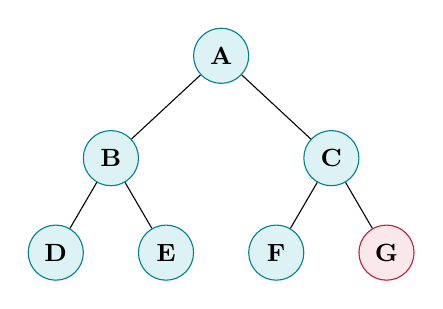
\begin{tikzpicture}[
  level 1/.style={sibling distance=2.8cm, level distance=1.3cm},
  level 2/.style={sibling distance=1.4cm, level distance=1.2cm},
  every node/.style={circle, draw=myteal, fill=hdrteal, inner sep=2pt, font=\small\bfseries, minimum size=0.7cm}
]
  \node {A}
    child {node {B}
      child {node {D}}
      child {node {E}}
    }
    child {node {C}
      child {node {F}}
      child [style={every node/.append style={draw=myred, fill=hdrred}}] {node {G}}
    };
\end{tikzpicture}
\end{tcolorbox}

\subsection{1. Breadth-First Search (BFS)}
\begin{itemize}[leftmargin=*, itemsep=3pt]
  \item \textbf{Mechanism:} Expands the root node first, then expands all successors of the root, then their successors. Implemented using a \textbf{FIFO (Queue)} frontier.
  \item \textbf{Completeness:} Complete (if branching factor $b$ is finite).
  \item \textbf{Time Complexity:} $O(b^d)$
  \item \textbf{Space Complexity:} $O(b^d)$ (all nodes kept in memory).
  \item \textbf{Optimality:} Optimal if step costs are uniform (equal to 1).
\end{itemize}

\subsection{2. Depth-First Search (DFS)}
\begin{itemize}[leftmargin=*, itemsep=3pt]
  \item \textbf{Mechanism:} Expands the deepest node in the current frontier. Implemented using a \textbf{LIFO (Stack)} frontier.
  \item \textbf{Completeness:} Incomplete in infinite state spaces or graphs with loops.
  \item \textbf{Time Complexity:} $O(b^m)$
  \item \textbf{Space Complexity:} $O(b \cdot m)$ (linear memory overhead!).
  \item \textbf{Optimality:} Non-optimal (may find a deeper solution before a shallow one).
\end{itemize}

\subsection{3. Depth-Limited Search (DLS)}
\begin{itemize}[leftmargin=*, itemsep=3pt]
  \item \textbf{Mechanism:} DFS with a pre-determined depth limit $l$. Nodes at depth $l$ are treated as if they have no successors.
  \item \textbf{Completeness:} Incomplete if $l < d$.
  \item \textbf{Time Complexity:} $O(b^l)$
  \item \textbf{Space Complexity:} $O(b \cdot l)$
  \item \textbf{Optimality:} Non-optimal if $l > d$.
\end{itemize}

\subsection{4. Iterative Deepening DFS (IDDFS)}
\begin{itemize}[leftmargin=*, itemsep=3pt]
  \item \textbf{Mechanism:} Combines the benefits of BFS (completeness/optimality) and DFS (linear memory). It calls DLS repeatedly with increasing depth limits $l = 0, 1, 2, \dots$
  \item \textbf{Completeness:} Complete (if $b$ is finite).
  \item \textbf{Time Complexity:} $O(b^d)$
  \item \textbf{Space Complexity:} $O(b \cdot d)$ (Linear space!).
  \item \textbf{Optimality:} Optimal if step costs are equal.
\end{itemize}

\subsection{5. Bidirectional Search}
\begin{itemize}[leftmargin=*, itemsep=3pt]
  \item \textbf{Mechanism:} Runs two simultaneous searches: one forward from initial state and one backward from goal state. Stops when frontiers intersect.
  \item \textbf{Completeness:} Complete if $b$ is finite and both searches are BFS.
  \item \textbf{Time Complexity:} $O(b^{d/2})$
  \item \textbf{Space Complexity:} $O(b^{d/2})$
  \item \textbf{Optimality:} Optimal if step costs are uniform.
\end{itemize}

% ===============================================================================
\section{Comparison of Search Strategies}
% ===============================================================================

\par\vspace{6pt}\noindent
{\renewcommand{\arraystretch}{1.45}%
\begin{tabularx}{\linewidth}{|B{3.0cm}|Y|Y|Y|Y|}
\hline
\textbf{Criterion} & \textbf{BFS} & \textbf{DFS} & \textbf{IDDFS} & \textbf{Bidirectional} \\
\hline
Completeness & Yes (if $b<\infty$) & No & Yes (if $b<\infty$) & Yes (if $b<\infty$) \\
\hline
Time Complexity & $O(b^d)$ & $O(b^m)$ & $O(b^d)$ & $O(b^{d/2})$ \\
\hline
Space Complexity & $O(b^d)$ & $O(b \cdot m)$ & $O(b \cdot d)$ & $O(b^{d/2})$ \\
\hline
Optimality & Yes (cost = 1) & No & Yes (cost = 1) & Yes (cost = 1) \\
\hline
Frontier Data Struct & FIFO Queue & LIFO Stack & LIFO Stack (Iterative) & Two FIFO Queues \\
\hline
\end{tabularx}}

\newpage
\begin{center}
  {\large\bfseries\color{myred} Quick Revision --- Module 2}\\[3pt]
  {\small\color{mydark} Solving Problems by Searching (Uninformed Search) $|$ OE-EC804A}
\end{center}
\noindent{\color{myred}\rule{\linewidth}{1.2pt}}
\vspace{4pt}

\begin{tcolorbox}[formulabox, title={\textbf{Key Concepts and Metrics at a Glance}}]
\renewcommand{\arraystretch}{1.35}
\begin{tabularx}{\linewidth}{B{4.5cm} X}
BFS Complexity & Time: $O(b^d)$, Space: $O(b^d)$ \quad (FIFO Queue, Complete, Optimal for step cost = 1) \\[4pt]
DFS Complexity & Time: $O(b^m)$, Space: $O(b \cdot m)$ \quad (LIFO Stack, Incomplete, Non-optimal) \\[4pt]
IDDFS Complexity & Time: $O(b^d)$, Space: $O(b \cdot d)$ \quad (Linear memory, Complete, Optimal) \\[4pt]
Bidirectional Search & Time: $O(b^{d/2})$, Space: $O(b^{d/2})$ \quad (Searches forward \& backward) \\[4pt]
Problem Components & Initial state $s_0$, Actions $Actions(s)$, Transition model $Result(s,a)$, Goal test, Path cost. \\
\end{tabularx}
\end{tcolorbox}

\begin{tcolorbox}[defbox, title={\textbf{One-Line Definitions}}]
  \begin{itemize}[leftmargin=*, noitemsep]
    \item \textbf{State Space:} Set of all valid states reachable from initial state.
    \item \textbf{Frontier:} Set of leaf nodes generated but not yet expanded.
    \item \textbf{Branching Factor ($b$):} Maximum number of successors for any node.
    \item \textbf{IDDFS:} Strategy running DLS with increasing limits $l=0,1,2,\dots$ combining BFS optimality with DFS space.
  \end{itemize}
\end{tcolorbox}

\begin{tcolorbox}[exambox, title={\textbf{Frequently Asked / Viva Questions}}]
  \begin{enumerate}[topsep=0pt, label=\textbf{Q\arabic*.}, itemsep=5pt]
    \item \Q{What are the 5 components of a formal problem definition?}
    Initial state, Actions, Transition model, Goal test, and Path cost.

    \item \Q{Compare BFS and DFS in terms of space complexity.}
    BFS requires $O(b^d)$ space (exponential), whereas DFS requires only $O(b \cdot m)$ space (linear).

    \item \Q{Why is IDDFS preferred over BFS for large state spaces?}
    IDDFS is complete and optimal like BFS, but uses linear space $O(b \cdot d)$ instead of exponential space $O(b^d)$.

    \item \Q{Why does node regeneration in IDDFS not incur high overhead?}
    Most nodes in a search tree are at the bottom level ($d$). Nodes at level $d$ are generated 1 time, level $d-1$ twice, etc., so total nodes generated $\approx \frac{b}{b-1} b^d$, which is asymptotically $O(b^d)$.

    \item \Q{What is the frontier in search algorithms?}
    The data structure (queue/stack) containing generated nodes that have not yet been expanded.

    \item \Q{When is BFS optimal?}
    BFS is optimal when all step costs are equal (uniform path cost).

    \item \Q{Explain the time and space complexity of Bidirectional Search.}
    Time and space complexities are both $O(b^{d/2})$ because two searches meet in the middle.

    \item \Q{What is Depth-Limited Search and why is it used?}
    DFS restricted to depth limit $l$. It prevents DFS from getting stuck in infinite paths.

    \item \Q{What is a Graph Search vs Tree Search?}
    Graph search maintains an `explored set` to avoid repeating states in looped graphs. Tree search does not.

    \item \Q{Define Completeness and Optimality.}
    Completeness: Guaranteed to find a solution if one exists. Optimality: Guaranteed to find the lowest-cost solution.
  \end{enumerate}
\end{tcolorbox}

\end{document}
